\section{Convolution and Design Matrix}

We need a good design matrix, containing data on the explanatory variables, to
be used in our linear models to explain as much variation in the observed fMRI
data as possible. We studied the design of the N-back experiment closely. fMRI 
scans were acquired while participants perform specified memory tasks. They 
are to respond to each letter shown as to whether it was the same as a 
pre-specified letter (0-back), the same as the immediately preceding letter 
(1-back), or the same as the letter shown two trials previously (2-back). 
For our subject, there were
three BOLD runs, each consisting of two blocks of 0-back, 1-back, or 2-back
working memory task. 

We examined the seven study conditions closely. The conditions are unusual from
what we are familiar with in that they are consisted of fractions of durations
and negative amplitudes. The first condition consists of
the start-cues, the second condition consists of the task targets (amplitudes
are all one), the third condition consists of the task non-target (the positive amplitude 
indicates correct identification of the target and the negative amplitude indicates the
non-response to the non-target), the fourth condition consists of end-cues, and
the fifth condition consists of durations of the two task blocks. There is no
information on what the sixth file mean, and the seventh condition consists of
the erroneous responses. All figures about convolution response are in the Appendix.

Since we were only familiar with convolution for block design, we initially used
only the condition one, four and five, which give us the start time, the
duration, and end time of the two task blocks. Due to the delay of signal after
the onset of neural activity, we make use of the hemodynamic response
function (HRF). The idea is to model the signal response as the convolution of
the stimulus function with the HRF. Convolving with stimulus timing allows us to
get idealized response as an explanatory variable (a regressor included in
design matrix). We bear in mind the limitations of this
design matrix due to its omission of trials within each of two task blocks. 

\begin{figure}[!h]
\centering
\begin{subfigure}{.33\textwidth}
  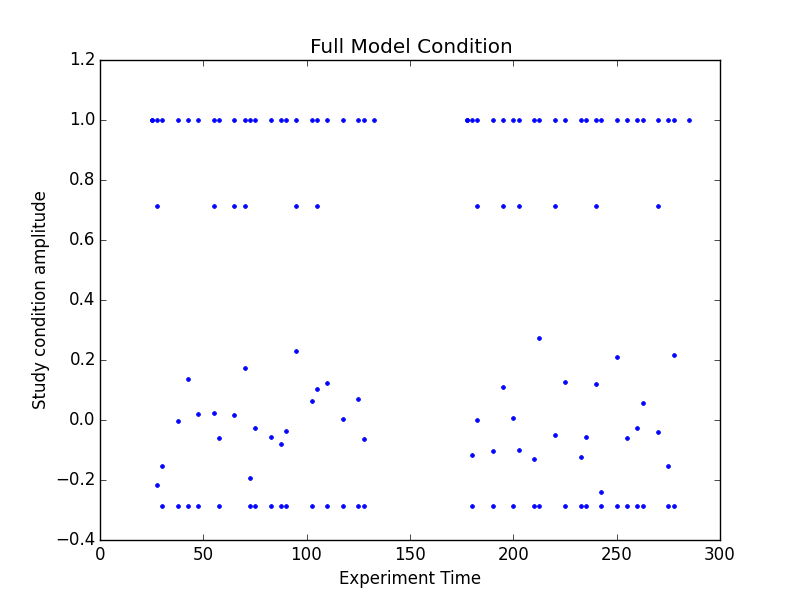
\includegraphics[scale=0.29]{task001_run001_full_points}
\end{subfigure}%
\begin{subfigure}{.33\textwidth}
  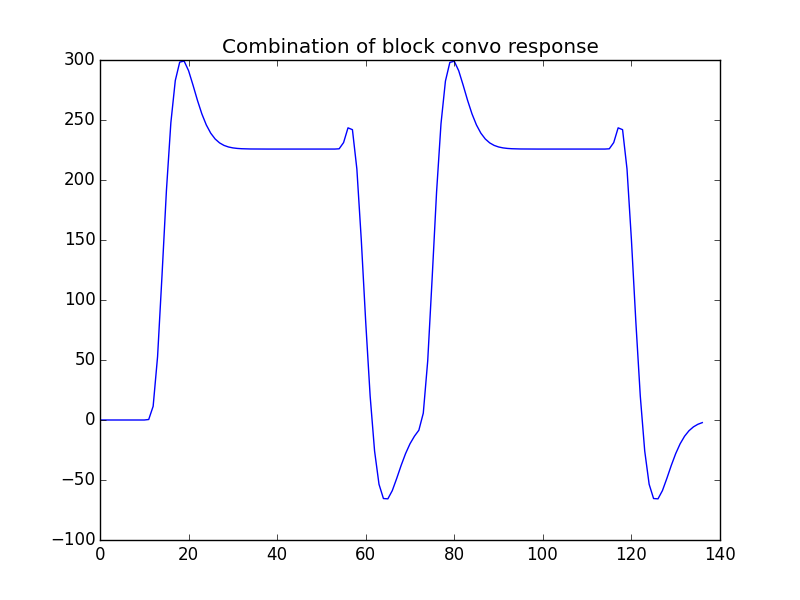
\includegraphics[scale=0.29]{combine_block_convo}
\end{subfigure}%
\begin{subfigure}{.33\textwidth}
  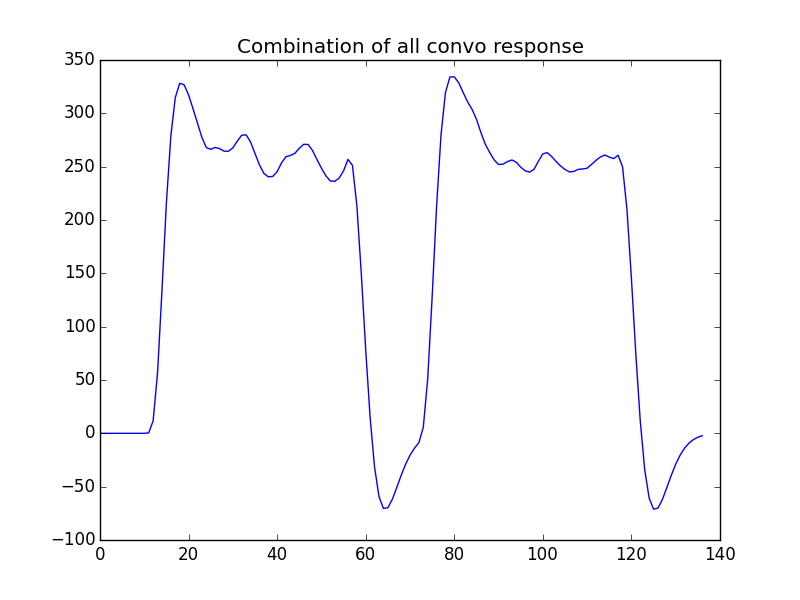
\includegraphics[scale=0.29]{combine_all_convo}
  \centering
\end{subfigure}
\caption{Combination of Block Design and Mixed Design\label{fig:Comb}}
\end{figure}

We are going to focus on the block design and mixed design in order to research
on the behaviors of individual voxels and the relationship between blood flows and 
task stimulus. 
